\subsection{Specific Applications}
\label{subsec:03_applications}

In this section we take a closer look at applications that are linked to cybersecurity on a secondary level: Here the Blockchain is not per se used to mitigate direct cybersecurity threats, but is used to make applications more robust, error-prone and less vulnerable. So the Blockchain does solve cybersecurity related issues, but in a more indirect way.

\subsubsection{Assessment Criteria}
Below we want to introduce different scenarios of applications (existing or proof-of-work drafts) for the Blockchain technology and apart from a brief introduction of the challenges and problems of this specific field, answer the following questions:
\begin{enumerate}
	\item What is the quality of this specific type of application regarding cybersecurity? 
	\item How do they make use of the Blockchain Technology?
	\item Is the BC really needed or could the problems be solved without it? 
\end{enumerate}
To answer question number 3 we are going to make use of the below schema presented by \citeauthor{Wust2017} in \cite{Wust2017}, that helps spliting real use cases from unnecessary ones.
\begin{figure}[ht!]
  \begin{center}
  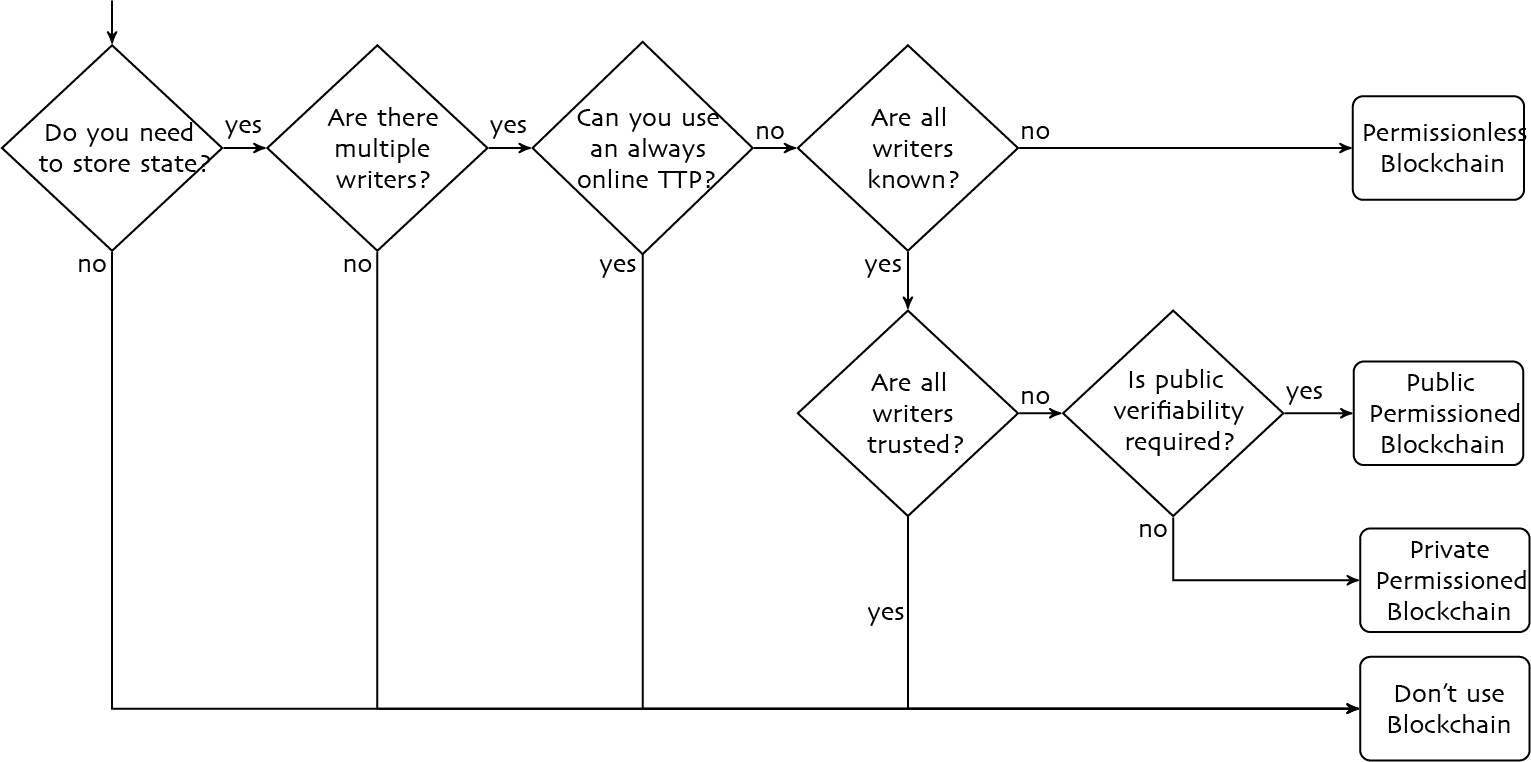
\includegraphics[scale=0.6]{Talk7/img/app/BCorNot}
  \end{center}
  \caption{Do you need a Blockchain?}
  \label{blockchain_or_not}
\end{figure}

\subsubsection{E-Voting}
Problem statement: Foundation of every successful democracy, must be accessible for all eligible citicens. Most common systems today are paper-based voting systems, have two major drawbacks. 1. Not scalable, 2. reliant on the procedural security of officials conducting their jobs. Various combinations exist, multiple security vulnerabilities pop up, that lead to an enourmous risk of election rigging and fraud. The Blockchain as system that is verifiable, scalable and tamper-proof, seems to be a good idea as solution. 

Idea for solution: Use the Blockchain technology for a transparent and incorruptible database that cannot have a single point of failure or be controlled by a single entity. Answers question 1

Several systems exist up till today. Not all rely on the same amount of integration of the Blockchain itself. Different use cases either in theory or in practice have already been tested on smaller county elections or within private organizations \cite{BenAyed2017}.

Estonian I-Voting System: Estonia was the first country where citizens where able to cast their vote online and with an electronic national identification card based on the Blockchain technology
Norwegian I-Voting System: In 2011 Norway used and eletronic remote voting system  for country council elections. The project was 2014 discontinued due to the fear of votes going public in case of a cyber attack.
New South Wales iVote System: In 2015 New South Wales used a hybrid blockchain based voting system.

General problems with the different systems: Single point of failure and closeness of critical parts of the code


Votebook (Quelle): Case study on Blockchain voting. No remote voting due to too many threats. Biggest problems: Authenticating user, voters computer as single point of failure DoS Attack.
Ressembles todays systems, based on paper voting and voting stations that have the Blockchain as backend.
System based on a permissioned, private blockchain with the voting stations as nodes
Follow my Vote (Quelle): Fundamentally different than Votebook. Each voter installs a local "Voting Box" on his computer, authenticating via uploaded official documents through the organization that holds the election. Each voter requests ballot online and votes. Allow for early voting as well as altering the vote later on. Based on  \citeauthor{Osgood2016} optimistic but flawed approach: Authentication and scaring off remote voters is a problem.

Vote Watchers (Quelle): Ressembles Votebook regarding the existence of paper ballots and real world voting stations. Each ballot contains three QR codes - 1 for BC address, 1 for ballot ID, 1 for election ID. Once ballot is scanned, the appropriate vote is sent to proper candidates unique address (like wallet) on an local offline BC of the voting station. After election is complete all data from local blockchain is put on a DVD and the machine is synchronized with the other machines for an evaluation of the voting results. 
Advantage: Offline use, allows no interference from hackers, at the same time the votes for each candidate can be checked in "real time" (??) by a blockchain explorer.
Uses BC only for tamper-proofness and public auditing, with everything else backed on paper ballots.

Proposition of \citeauthor{Osgood2016} is therefore a system that still relies upon paper ballots, where people have to authenticate by showing up in real life at a real world voting booth, that uses the Blockchain for its tamper-proofness and ability to account as an auditing system

Proposition of \citeauthor{BenAyed2017}:
Tries to fulfill the following criteria: 1 (Authentication)Only people already registered to vote can cast votes. The system does not include registration and authentification has to be done externally. 2 (Anonymity) The system will not allow any links between voters votes and identities. 3 (Accuracy) Votes must be accurate and votes can neither be changed, nor duplicated, nor removed. 4 (Verifiablity): The system is verifiable to make sure all votes are counted correctly
Limitations: User as single point of failure is still a problem and inability to change the vote once casted.

General problem: Spotlight too much on the developed part of the world instead of focussing regions where a trust-less system is really used.

Question 3: 
In a voting scenario the authorities need the state of an election to be stored at all times during an election. For one, because of verifiability of the results in the end, but also because of any security related problems that could cause a shutdown of one or multiple of the voting stations. The writers are the voters and need to be known or in any way authenticated by a third party. In this scenario only an organization that has access to all the data is able to do that. In most cases this leaves only the government as a real option. In this scenario the voters per definition do not trust other voters as everyone is assumed to have a different desired output. 
According to the diagram by  \citeauthor{Wust2017} the use of Blockchain technology therefore only makes sense in country where the government is not a thrusted third party. In which case a public permissioned Blockchain would be the best solution.
Nevertheless, it is the role of the government that causes the dilemma itself. If the non-existing trust in the government is the justification for the use of the Blockchain, the question arises whether the government can be trusted regarding the authentication of the voters. Even though a systematic rigging is harder to achieve with this approach, the problem remains at hand. 

While the Blockchain does seem to be perfect for a voting situations, its justification remains questionable. Especially, because it still leaves the most important point of failure unprotected: The user himself. Even the most tamperproofed, blockchain-based voting system does not prevent hackers from a man-in-the-middle attack from a compromised end-device. 

To sum this chapter up: Many of the desired e-Voting properties that the Blockchain technology provides have trade-offs. The aspect of privacy is just one of many. On the other hand, no system has yet been proposed that has been shown to be secure, verifiable and private at the same time. The question of authentifiation comes into play as additional point of failure of the concept.
Therefore: If a online trusted third party exists, the use of the blockchain is not necessary. If the government is trusted as far as the authentification of the voters goes, a public permissioned Blockchain can be a good fit. However the security of the system then relies on the interity of the validators. 
If the government is trusted not at all, there exists no solution that overcomes that systematic flaw in a countries governance.

The Blockchain can therefore be a solution if the question of authentification can be answered satisfactorily. Otherwise a traditional paper based voting system is as good as voting system including Blockchain based systems or systems that base on a trusted third party.

\subsubsection{Autonomous Vehicles}
Smart vehicles are increasingly connected to infrastructure such as traffic management systems, other vehicles and also more generally the Internet, thus making the vehicles part of the Internet of Things (IoT). This developement brings obvious advantages, but also many challenges, especially in the area of cybersecurity. Malicious attacks on a vehicle endanger not only the vehicles data and the passengers of the vehicle itself, but also other road users. And while many conventional security and privacy methods exist to reduce the risk of an attack they tend to be ineffective due to centralization, unscalability and unsecure communication architectures \cite{DorriSteger2017}.
Meanwhile the challenges on a secure and yet scalable system for connecting self-driving vehicles with not only each other, but also with other participating entities such as power stations and traffic management systems are many: They need to be scalable, secure and tamper-proof, private but at the same time accessible to specific other entities

The Blockchain offers solutions by design to before mentioned problems: It works decentralized and is tamperproof at all times. The idea of connecting autonomous vehicles to a system based on the Blockchain technology immediately comes to mind.
At the same time its design does not include the aspect of privacy per se. The mentioned challenges are tackled in various approaches. Therefore various approaches exist to connect self-driving vehicles with a blockchain-based architecture.

Idea of \citeauthor{DorriSteger2017}: A decentralized privacy-preserving and secure blockchain-based architecture for the smart vehicle ecosystem. It bases on its own Blockchain called Lightweight Scalable Blockchain (LSB) that minimizes the overhead and increases scalablility as well as the throughput.
It consists of clusters of nodes which are connected to the system via their Cluster Heads (CHs) also called Overlay Block Managers (OBMs).  All Transactions are broadcast to and verified by the OBMs. 
To ensure the users privacy, each vehicle is equipped with an internal vehicle storage to store sensitive data. It is the vehicle owner himself, who defines which data is provided to third parties and which data is not.
The complete system looks the following way: Each vehicle is part of the Internet of Things and hence connected to the Internet. Through this link the vehicle is connected to an overlay consisting of various OBMs that form the nodes of the Blockchain based system.
The vehicle generates single signature transactions in pre-defined time intervalls containing the signed hash of the data stored in the in-vehicle storage. This transaction is sent to and validated by the closest OBM, which finally stores it in the Blockchain That way at all times, the users datas integriy can be validated.
To make certain Public Keys identifiable in the real world a trusted third party is involved and the mechanism is centralized. This is needed in the case of service centers and software providers.
Through this ecosystem various standard applications can be leveraged, such as remote software updates, vehicle insurance, Smart Charging and Vehicle Sharing Devices.

Idea of \citeauthor{Rowan2017}: Their paper focusses on the communication between two vehicles and vehicles and infrastructures through side-channels such as visible light and acoustic signals. To solve the problem of the limited data throughput while trying to securely validate the other communication partner, centralized approaches were discarded due to the high number of manufacturers and standards. Instead \citeauthor{Rowan2017} propose a blockchain based domain name system an dpublic key infrastructure, as they do not require centralisation in order to push data into the distributed database. 
The blockchain based approach was chosen as most promising way of storing public keys due to its robustness and security regarding large scale attacks. 
In the case of \citeauthor{Rowan2017} the Blockstack (Quelle) software was used. It is an open source, per reviewed application stack implementation that provides identity, naming, storage and authentication services. It ressembles a distributed database without central management.
To establish a session between two parties, the paper now proposes a new approach, designed to integrate the security and communications requirements in authonoumous vehicle communication: Based on the TLS 1.2 handshake it differs only in one point: To minimize the throughput requirement it uses a blockchain distributed hashtable. 
All in all the systems advantages are huge:
It has a very small required throughput, it is able to locate the vehicle being communicated with, the vehicle can be authenticated using a certificate, the encryption is symmetric using PKI architecture.

The main use of the Blockchain in this case is therefore its use for the handshake itself. The communication in this scenario needs to be extremeley fast and include as little overhead as possible and work in the absence of any wireless or any cantralized infrastructure. To make this possible, the handshake, that authenticates the involved partners and establishes a secure session, makes use of the Blockchain in the form of a decentralized Domain Name Service.

In this case the Blockchain is used as a way to replace the need for a central authority when authenticating another vehicle. By creating a decentralized Name Service that binds the licence plate value and an identity together with a certificate it is able to create a good base for a secure session between two verifiably trusted vehicles.

However the paper does give little information about, where the different nodes of the blockchain lie and how they communicate. It is only assumed that the vehicles are the nodes.

Autonomous vehicles communicating with each other using the Blockchain as a base for authentication seems like a good use case. The application requires to store the state of the data, there are multiple writers, that are not trusted and online access to a central authority or a trusted third party can not be assumed at all times. Applying the flow-chart by \citeauthor{Wust2017}, this use case calls for a private permissioned Blockchain. 
According to the paper by \citeauthor{Rowan2017} this is exactly what was done. 
Nevertheless the use of any private permissioned blockchain requires central registration through a trusted third party in the first place. And it is this very point that raises the following question: One main reason for the use of the Blockchain as a decentralized public key domain name service in favor of a central authority, was the fact, that "a centralized system would not find favour due to the multitude of manufacturers, political regions and vehicle types" \cite{Rowan2017}. Why would this be different when issueing certificates?
In the end we still run into the problem that we need an external party that trustfully binds real goods to a public key in the digital world. 
To use the Blockchain to create a decentralized name service is a good and useful idea as it does not rely on the Internet, but the underlying assumption that it does get rid of any central authority is flawed.

Did i understand it right???

\citeauthor{Sharma2017} identifies several challenges when creating a network for autonomous vehicles.



\begin{itemize}
	\item \cite{Sharma2017}
\end{itemize}
\subsubsection{Personal Data Protection and Patient Monitoring}
\begin{itemize}
	\item \cite{Zyskind2015}
	\item \cite{Yue2016}
	\item \cite{Azaria2016}
	\item \cite{Fotiou2016}
	\item \cite{Zhang2017}
	\item \cite{Zhang2018}
	\item \cite{Esposito2018}
	\item \cite{Ekblaw2016}
	\item \cite{Cao2019}
\end{itemize}
\subsubsection{Smart Cities \& IoT}
\begin{itemize}
	\item \cite{Biswas2016}
	\item \cite{Mylrea2017}
	\item \cite{Liang2018}
	\item \cite{Dorri2017a}
	\item \cite{Shafagh2017}
\end{itemize}

